\section*{Direction 1. How the feeding law changes coexistence and enrichment}

\subsection*{Abstract}
We kept the coursework prey growth law and compared five ways predators consume prey. In all five models, positive initial populations remain positive and ultimately bounded. The feeding laws differ in how many coexistence equilibria they admit and how those equilibria respond to increasing carrying capacity. For prey-dependent feeding, a feasible predator break-even density gives a unique coexistence branch and an upward stability crossing as carrying capacity increases. Predator interference can give three equilibria. For ratio-dependent feeding, we prove a necessary and sufficient condition on prey growth for enrichment to decrease the equilibrium trace across all admissible intakes. In four algae--rotifer experiments, the best one-step predictor changed when the fitting bounds were widened.

\subsection*{Results}
Let $x$ and $y$ be prey and predator density, $K$ the prey carrying capacity, $e$ the conversion efficiency, and $d$ the predator mortality rate. The original equations are
\[
 \dot x=xq(x,K)-P(x,y),\qquad \dot y=eP(x,y)-dy,\qquad
 q(x,K)=r(1-x/K)(1+\alpha x).
\]
All shared coefficients $r,K,\alpha,e,d$ are positive. The weak Allee factor $1+\alpha x$ acts on prey growth. The per-capita growth rate rises near zero precisely when $\alpha K>1$. The coursework uses $P_0=mxy/(\beta+y)$, equivalently $axy/(1+cy)$ with $a=m/\beta$ and $c=1/\beta$.

\begin{center}\small
\begin{tabular}{@{}lll@{}}
\toprule
Model & Total consumption $P(x,y)$ & What fixes positive coexistence \\
\midrule
P0\quad Foraging arena & $axy/(1+cy)$ & An affine predator nullcline \\
P1\quad Mass action & $axy$ & A fixed prey density \\
P2\quad Holling type II & $axy/(1+bx)$ & A fixed prey density \\
P3\quad Beddington--DeAngelis & $axy/(1+bx+cy)$ & An affine predator nullcline \\
P4\quad Ratio-dependent Holling II & $axy/(x+cy)$ & A fixed predator-to-prey ratio \\
\bottomrule
\end{tabular}
\end{center}

For P0--P3, let $\mathcal R=eaK/[d(1+bK)]$, with $b=0$ where absent. When $\mathcal R\leq1$, every positive trajectory converges to $(K,0)$. When $\mathcal R>1$, both species persist uniformly. In this regime P1/P2 have one positive equilibrium. P2 requires $ea>db$ for a finite positive break-even density. P0/P3 can have three, with a saddle between the outer branches. For example, P0 with $r=e=d=1$, $K=8$, $\alpha=1/2$, $a=9/2$, and $c=8/3$ has attracting equilibria $(1,21/16)$ and $(3,75/16)$ separated by the saddle $(2,3)$. P4 has at most two positive equilibria. A positive predator invasion rate at $(K,0)$ can coexist with an open basin of joint extinction.

When $\alpha>0$ and $u=1/(ea/d-b)>0$, the P1/P2 coexistence branch exists for $K>u$. Increasing $K$ carries this branch through a supercritical Hopf bifurcation, creating nearby stable oscillations. For P4 the trace decreases on every positive-determinant branch under the same prey growth. P0 and P3 each allow either trace direction. Separate exact examples give fold, Hopf and Bogdanov--Takens bifurcations in P0, P3, and P4. A Bogdanov--Takens point has a double zero eigenvalue and two independent unfolding parameters. For example, P0 has a supercritical Hopf bifurcation at $(1,1)$ when $(r,K,\alpha,a,c)=(9/25,6,7/3,2,1)$ and $e=d=1$. At this point $\Delta=1/4$ and, as $r$ varies, $dT/dr=-1/6$.

\clearpage
\subsection*{Figures and tables}
\textbf{A controlled comparison.}
We matched the intake of a rare predator at $x=10$ to $0.9$ in all five laws. The common parameters were $(r,K,\alpha,e,d)=(0.7,10,0.12,0.6,0.3)$. For P0--P3, $b=0.15$ and $c=0.2$ where present and $a=0.09(1+10b)$. For P4, $a=0.9$ and $c=2$. This specifies the same invasion rate at the reference capacity while allowing distinct responses away from it.

\begin{center}
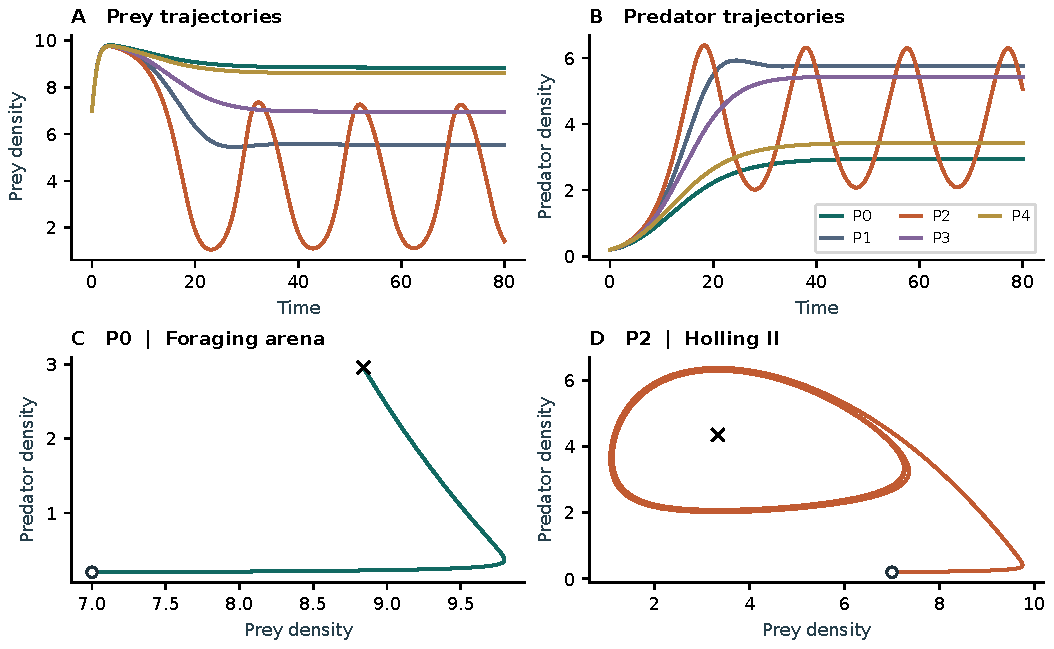
\includegraphics[width=.91\linewidth]{d1/figures/matched_dynamics.pdf}
\end{center}
{\small\textbf{Figure 1.1.} All trajectories start at $(7,0.2)$. The top panels track densities over time. The lower panels trace P0 and P2 in the population plane. The cross marks coexistence. P0 approaches its equilibrium, whereas P2 oscillates around an unstable equilibrium.}

\begin{center}\small
\begin{tabular}{@{}lrrrrr@{}}
\toprule
 & \multicolumn{3}{c}{Matched synthetic comparison} & \multicolumn{2}{c}{Observed one-step error}\\
\cmidrule(lr){2-4}\cmidrule(l){5-6}
Model & $x_*$ & $y_*$ & Largest $\operatorname{Re}\lambda$ & Primary bounds & Wider bounds\\
\midrule
P0 & 8.841 & 2.957 & $-0.1416$ & 0.867367 & \textbf{0.868031}\\
P1 & 5.556 & 5.761 & $-0.2204$ & 0.906098 & 0.906096\\
P2 & 3.333 & 4.356 & $+0.0389$ & 0.906112 & 0.906097\\
P3 & 6.958 & 5.437 & $-0.2615$ & 0.867378 & 0.868132\\
P4 & 8.593 & 3.437 & $-0.1506$ & \textbf{0.857747} & 0.870391\\
Last observation & & & & 1.040276 & 1.040276\\
\bottomrule
\end{tabular}
\end{center}
{\small\textbf{Table 1.1.} The last two columns use four observed algae--rotifer chemostat experiments (\href{https://doi.org/10.1038/s41586-019-1857-0}{Blasius et al.}, \textit{Nature} 577, 226--230, 2020). Each experiment was held out in turn, giving 861 observed intervals. Each prediction started from the latest observed populations. We averaged prey and predator errors after scaling by training variation, then weighted the four experiments equally. Smaller scores are better. Widening every parameter range tenfold at both ends changed the best mean score from P4 to P0. These data leave the feeding law unresolved.}

\clearpage
\textbf{Two local stability crossings.}
The following example uses $g(x)=1+x^2$ in $q(x,K)=g(x)(1-x/K)$ to explore what can happen outside the coursework growth law. Fix $e=d=1$ and $p(z)=110/(65+54z)$, where $z=y/x$. Its unique positive branch satisfies
\[
 y=\tfrac56x,\quad
 K=\frac{6x(1+x^2)}{1+6x^2},\quad
 T=-\frac{(3x^2-1)(4x^2-1)}{12(1+x^2)},\quad
 \Delta=\tfrac{3}{88}-\tfrac{9}{22}T.
\]
Here $T$ is the Jacobian trace and $\Delta$ its determinant. Both $K'(x)$ and $\Delta$ are positive along the branch. Thus the signs of the two trace factors give the stability intervals directly.

\begin{center}
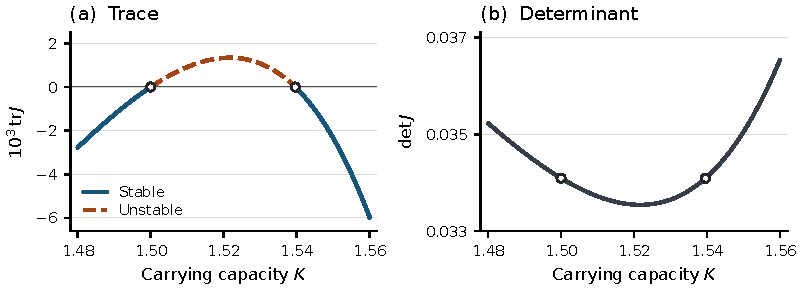
\includegraphics[width=.89\linewidth]{d1/figures/stability_crossing.pdf}
\end{center}
{\small\textbf{Figure 1.2.} With the same intake throughout, coexistence loses local stability at $K=3/2$ and regains it at $K=8/(3\sqrt3)$. The corresponding trace slopes are $1/9$ and $-3\sqrt3/32$. A Hopf classification for these two crossings requires the nonlinear coefficient.}

\medskip\noindent\textbf{Two long-term outcomes under one parameter set.}
Return to P4 with the coursework factor $g=1+x/2$. Set $K=8$, $a=4/5$, $c=8/15$, $e=1$, and $d=1/5$. The prey coordinates of the two positive equilibria are $3\pm\sqrt7$. The lower equilibrium is a saddle and the upper one attracts nearby trajectories.

\begin{center}
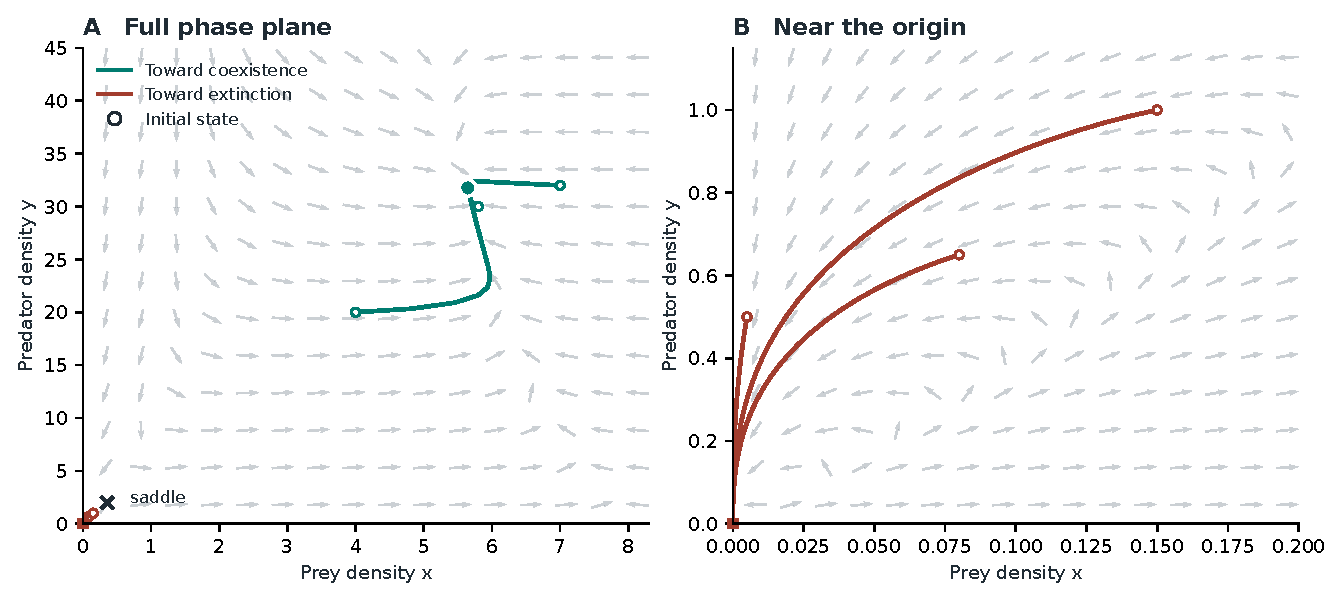
\includegraphics[width=.86\linewidth]{d1/figures/ratio_basins.pdf}
\end{center}
{\small\textbf{Figure 1.3.} Three initial conditions approach coexistence and three approach joint extinction. In the region $0<x<0.01$, $u=8y/(15x)>10$, the equations give $\dot x/x<-0.35$ and $\dot u/u>0.23$. This region is forward invariant. There $x\to0$, $u\to\infty$ and $\dot y/y\to-0.2$, proving convergence to extinction for an open set of initial states.}

\clearpage
\subsection*{Mathematical proofs}
\textbf{Why the five laws give different equilibrium counts.}
For P0--P3 write $D=1+bx+cy$, putting absent coefficients equal to zero, and set $A=ea/d-b$. Predator break-even at a positive equilibrium gives $1+cy=Ax$. The prey equation then gives $y=exq/d$. Thus P1/P2 fix $x=1/A$ when $A>0$ and $K>1/A$. P0/P3 require a root of the cubic
\[
 H(x)=\frac{ce}{d}xq(x,K)-Ax+1=0,\qquad 1/A<x<K.
\]
For the P0 example above, $H=-(x-1)(x-2)(x-3)/6$. At positive roots $\Delta=-dqxH'/D$. The middle root has negative determinant, while the two outer roots have positive determinant and negative trace by substitution. In P4 the same predator equation fixes $\rho=y/x=(ea/d-1)/c$. The prey equation reduces to $q(x,K)=\rho d/e$, a quadratic level equation. The common identity $(ex+y)'=exq-dy$ explains the shared bound despite these different geometries. For any $0<\eta\le d$, $(ex+y)'+\eta(ex+y)\le ex(q+\eta)$, whose supremum over $x\ge0$ is finite.

\medskip\noindent\textbf{Reciprocal-curvature theorem.}
Fix $e,d>0$ and a prey density $s$ in an open interval $I\subset(0,\infty)$. Let $g\in C^2(I)$ with $g,g'>0$. Consider the original-time system
\[
 \dot x=xg(x)(1-x/K)-yp(y/x),\qquad \dot y=y[ep(y/x)-d].
\]
The condition $(1/g)''(s)\ge0$ is equivalent to the following property. For every positive, strictly decreasing $p\in C^1(0,\infty)$, every $K_0>0$, and every $v>0$ giving an equilibrium $(s,v)$ with $\Delta>0$ at $K_0$, the trace along its local branch satisfies $dT/dK<0$ at $K_0$. Only $K$ varies on a given branch.

\medskip\noindent\textit{Proof.}
At coexistence $p(\rho)=d/e$, so $\rho$ and $Q=\rho d/e$ are fixed and $q(x,K)=Q$. Direct differentiation of the original field gives
\[
 T=xq_x+Q+\rho(\rho+e)p'(\rho),\qquad
 \Delta=e\rho p'(\rho)xq_x .
\]
Strict decrease gives $p'(\rho)\le0$. A positive determinant forces $p'(\rho)<0$ and $q_x<0$, so $x_K=-q_K/q_x>0$ by implicit differentiation. Put $E=xg'/g$, $D_0=g-(1+E)Q$, and $U=g/(1+E)$. Substituting $x/K=1-Q/g$ gives $xq_x=-D_0$. Thus $0<Q<U$ and
\[
 T_K=x_KL(Q),\qquad L(Q)=QE'-g',\qquad
 L(0)=-g',\quad L(U)=-\frac{s g^2}{1+E}(1/g)''(s).
\]
The endpoint expressions use $x=s$. If reciprocal curvature is nonnegative, the affine function $L$ is negative at $0$ and nonpositive at $U$, hence strictly negative throughout the open interval. Conversely, when curvature is negative, $L$ has an interior zero and takes both signs. To realize any interior load, choose $\rho=eQ/d$, $K_0=s/(1-Q/g(s))$, and $p(z)=(2d/e)/(1+z/\rho)$. Then $q(s,K_0)=Q$, $p(\rho)=d/e$, $p'(\rho)<0$, and $D_0>0$. These choices yield $\Delta>0$ and all three possible trace slopes at the prescribed density.\hfill$\square$

\clearpage
\textbf{Application to the original prey growth.}
For $g=r(1+\alpha x)$ with $\alpha>0$,
\[
 (1/g)''=\frac{2\alpha^2}{r(1+\alpha x)^3}>0.
\]
The P4 trace therefore decreases with $K$ at every positive-determinant coexistence equilibrium. For prey-dependent intake $f(x)$ the predator equation instead fixes $u$ through $f(u)=d/e$. Substitution in the Cartesian trace yields
\[
 T_K=\frac{u g(u)}{K^2}\left(2+\frac{u g'(u)}{g(u)}-\frac{u f'(u)}{f(u)}\right).
\]
Since increasing concave $f$ with $f(0)=0$ satisfies $uf'(u)\le f(u)$, P1/P2 have $T_K>0$. In the mixed cases the equilibrium itself moves. At the identical point $x=y=e=d=1$, $K=2$, $g=1+x$, set $a=1+b+c$. The P0 choices $(b,c)=(0,1),(0,2)$ give $T_K=1/12,-1/6$. The P3 choices $(1,1),(1,3)$ give $1/4,-23/100$. All four determinants are positive.

\subsection*{Python code}
The following SymPy example computes the Cartesian Jacobian, substitutes the equilibrium branch of Figure~1.2, and checks the trace, determinant, and trace slope at the first crossing.

\begin{lstlisting}[language=Python,basicstyle=\ttfamily\footnotesize]
import sympy as sp

x, y, K = sp.symbols("x y K", positive=True)
feed = 110*x*y / (65*x + 54*y)
field = sp.Matrix([x*(1 + x**2)*(1 - x/K) - feed, feed - y])
J = field.jacobian((x, y))
capacity = 6*x*(1 + x**2) / (1 + 6*x**2)
branch = {y: sp.Rational(5, 6)*x, K: capacity}
trace = sp.factor(J.trace().subs(branch))
slope = sp.diff(trace, x) / sp.diff(capacity, x)
first = sp.Rational(1, 2)
result = tuple(sp.simplify(f.subs(x, first))
               for f in (trace, J.det().subs(branch), slope))
assert result == (0, sp.Rational(3, 88), sp.Rational(1, 9))
print(result)
\end{lstlisting}
The output is $(0,3/88,1/9)$. The broader symbolic check passed all 12 identities, including the second crossing and the mixed-model slopes above.

\subsection*{Lean verification results}
Lean 4.19.0 with Mathlib v4.19.0 checked 44 public declarations. The verified results include the Cartesian equilibrium and Jacobian, both directions of the reciprocal-curvature criterion, the three Holling II witnesses at negative curvature, and the affine-growth application to P4. For Figure~1.2, Lean verified the equilibrium $(1/2,5/12)$ and the exact values $T=0$, $\Delta=3/88$, $(1/g)''=-32/125$, and $T_K=1/9$. The verification takes the trace along a local solution of the original equilibrium equations.

The second crossing follows from the branch formula in Figure~1.2 and symbolic differentiation. The trajectories and prediction errors come from the numerical comparisons.
